% Copyright (c) 2005-2009 Nokia Corporation
%
% Licensed under the Apache License, Version 2.0 (the "License");
% you may not use this file except in compliance with the License.
% You may obtain a copy of the License at
%
%     http://www.apache.org/licenses/LICENSE-2.0
%
% Unless required by applicable law or agreed to in writing, software
% distributed under the License is distributed on an "AS IS" BASIS,
% WITHOUT WARRANTIES OR CONDITIONS OF ANY KIND, either express or implied.
% See the License for the specific language governing permissions and
% limitations under the License.

\newlength{\screenwidth}
\setlength{\screenwidth}{0.3\textwidth}
\label{sec:appuifw}

\section{\module{appuifw} ---
	 Interface to the S60 GUI framework}

\declaremodule{standard}{appuifw}
\platform{S60}
\modulesynopsis{Interface to the S60 GUI framework}

The \module{appuifw} module offers an interface to the S60 UI application
framework. \figurename~\ref{fig:ui-overview} provides an overview of
the Python for S60 environment for UI application programming.

\note{The services of this interface may only be used in the context of 
the main thread, that is, the initial thread of a UI application script.}

\begin{figure}
\centering
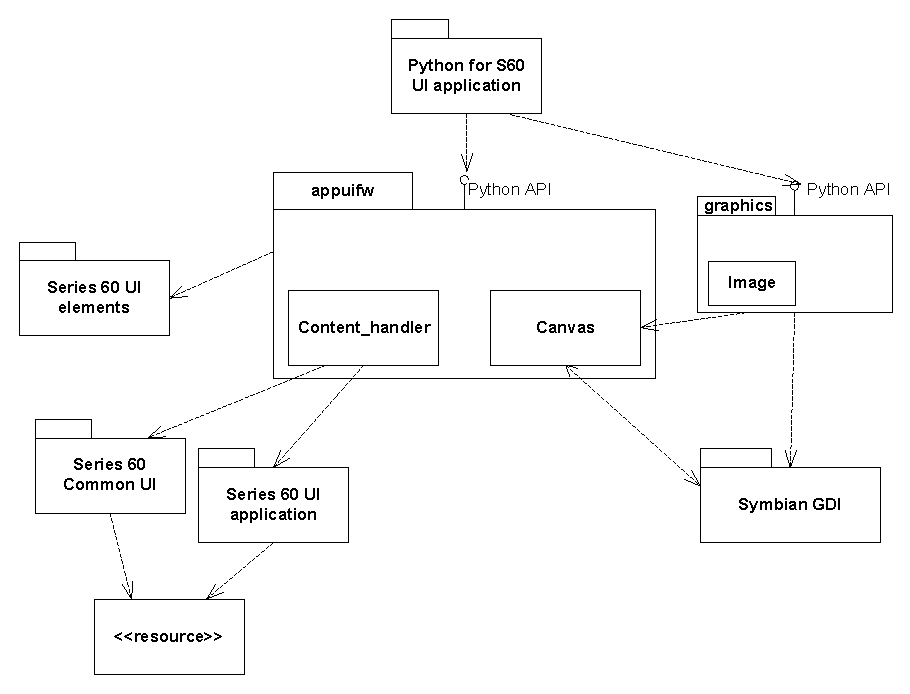
\includegraphics[width=\textwidth]{ui-overview}
\caption{Python for S60 UI environment overview}
\label{fig:ui-overview}
\end{figure}

\subsection{Basics of appuifw Module}
\label{subsec:basics}
Figure \ref{fig:normal-uilayout} shows the layout of a S60 application 
UI in the normal screen mode and a summary of how it relates to the services 
available at the \module{appuifw} API. For alternative layouts, see 
Figure \ref{fig:alternate-uilayouts}.

\begin{figure}
\centering
%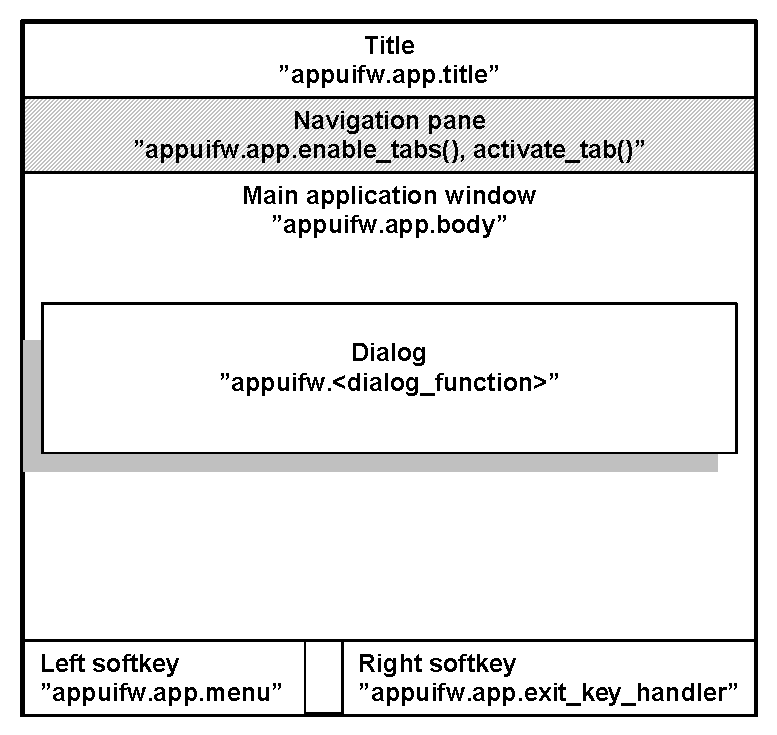
\includegraphics[width=0.7\textwidth]{screen-parts}
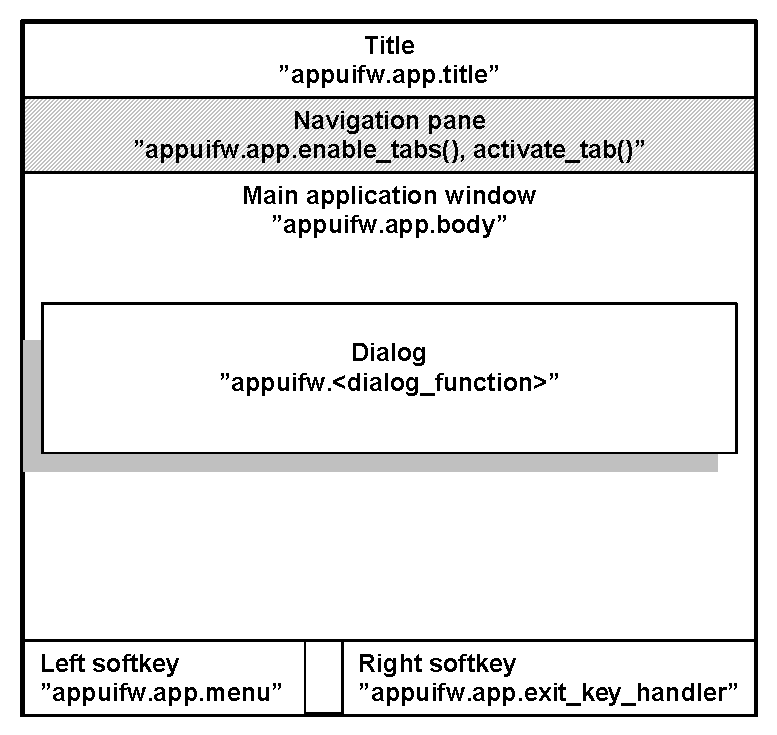
\includegraphics{screen-parts}
\caption{The different parts of the screen when using the 'normal' layout}
\label{fig:normal-uilayout}
\end{figure}

\begin{figure}
\centering
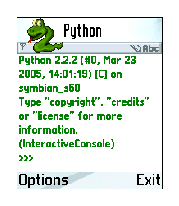
\includegraphics[width=\screenwidth]{layout-normal}
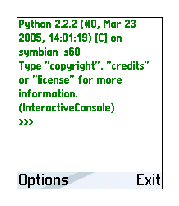
\includegraphics[width=\screenwidth]{layout-large}
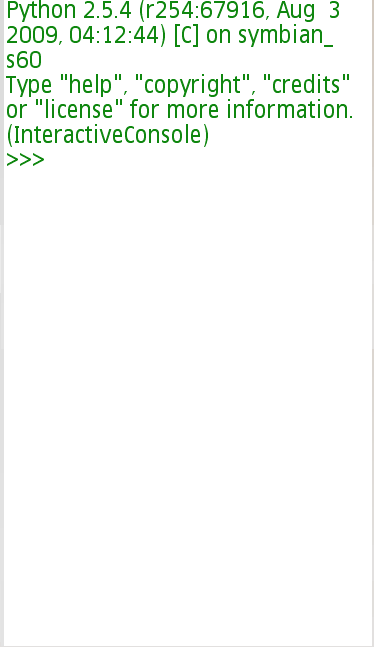
\includegraphics[width=\screenwidth]{layout-full}
\caption{UI layouts. left: 'normal', middle: 'large', right: 'full'}
\label{fig:alternate-uilayouts}
\end{figure}

The main application window may be set up to be occupied by a UI control.

A multi-view application can show the different views as tabs in the 
navigation pane and react as the users navigate between tabs. 

Dialogs always take precedence over the usual UI controls and appear on top 
of them.

UI controls are implemented as Python types. These types are available:

\begin{itemize}
\item \class{Text}
\item \class{Listbox}
\item \class{Canvas}
\end{itemize}
UI controls appear on the screen as soon as an instance of the corresponding 
Python type is set to the body field (\var{app.body}) of the current application UI.

\class{Form} is a versatile dialog implemented as a type.

The \class{Content_handler} type facilitates interfacing to other UI
applications and common high-level UI components. It is based on the
notion that designated handlers can reduce UI application interaction
to operations on MIME-type content.

The following dialogs are implemented as functions:

\begin{itemize}
\item \function{note}
\item \function{query}
\item \function{multi_query}
\item \function{selection_list}
\item \function{multi_selection_list}
\item \function{popup_menu}
\end{itemize}
A dialog becomes visible as soon as the corresponding Python function has 
been called. The function returns with the eventual user input or 
information on the cancellation of the dialog. \class{Form} is an 
exception; it is shown when its \method{execute} method is called.

\subsection{Softkeys}
\label{subsec:softkeys}
The softkeys are managed by the underlying S60 Platform. When no
dialog is visible, the right softkey is bound to application exit and
the left one represents an Options menu. Python for S60 offers
an interface for manipulating the menu and for binding the Exit key to
a Python-callable object (see Section \ref{subsec:application}). 

The native code that implements a dialog also manages the softkeys of the 
dialog, typically OK and Cancel. When the user input needs to be validated 
before accepting it and dismissing the dialog, it is best to use 
\class{Form}.

\subsection{Module Level Functions}
\label{subsec:module}
The following free functions - functions that do not belong to any class 
- are defined in the \module{appuifw} module:

\begin{funcdesc}{available_fonts}{}
Returns a list (Unicode) of all fonts available in the device.
\end{funcdesc}

\begin{funcdesc}{touch_enabled}{}
Returns 'True' if the device supports touch input, 'False' otherwise.
\end{funcdesc}

\begin{funcdesc}{query}{label, type\optional{, initial_value}}
Performs a query with a single-field dialog. The prompt is set to 
\var{label}, and the type of the dialog is defined by \var{type}. The 
value of \var{type} can be any of the following strings:

\begin{itemize}
\item \code{'text'}
\item \code{'code'}
\item \code{'number'}
\item \code{'date'}
\item \code{'time'}
\item \code{'query'}
\item \code{'float'}
\end{itemize}

The type of the optional \var{initial_value} parameter and the 
returned input depend on the value of \var{type}:

\begin{itemize}
\item For text fields, (\code{'text'}, \code{'code'}) it is Unicode
\item For number fields, it is numeric
\item For date fields, it is seconds since epoch rounded down to the nearest local midnight
\end{itemize}

A simple confirmation query and time query take no initial value and return 
\code{True/None} and seconds since local midnight, correspondingly. All 
queries return \code{None} if the users cancel the dialog. 

For \code{'float'} query the \var{initial_value} setting has no 
effect.
\end{funcdesc}


\begin{funcdesc}{multi_query}{label_1, label_2}
A two-field text (Unicode) input dialog. Returns the input values
as a 2-tuple. Returns \code{None} if the users cancel the dialog.
\end{funcdesc}

\begin{funcdesc}{note}{text\optional{, type\optional{, global}}}
Displays a note dialog of the chosen type with \var{text} 
(Unicode). The default value for \var{type} is \code{'info'}, which is 
automatically used if \var{type} is not set. \var{type} can be one of 
the following strings: \code{'error'}, \code{'info'} or 
\code{'conf'}. 

If \var{global} (integer) is any other value than zero a global note is 
displayed. A global note is displayed even if the Python application calling 
this function is in background. The same set of \var{type}s is supported as in 
standard note.
\end{funcdesc}

\begin{funcdesc}{popup_menu}{list\optional{, label}}
A pop-up menu style dialog. \var{list} representing the menu 
contents can be a list of Unicode strings or a list of Unicode string pairs 
(tuples). The resulting dialog list is then a single-style or a double-style 
list. A single-style list is shown in full; whereas a double-style list 
shows the items one at a time. Returns \code{None} if the user cancels the 
operation.
\end{funcdesc}

\begin{funcdesc}{selection_list}{choices\optional{, search_field=0}}
Executes a dialog that allows the users to select a list item and
returns the \var{index} of the chosen item, or \code{None} if the
selection is cancelled by the users. \var{choices} is a list of
Unicode strings.
\var{search_field} is \code{0} (disabled) by default and is optional. Setting it to \code{1} enables a search field (find pane) that facilitates searching for items in long lists. If enabled, the search field appears after you press a letter key.
\end{funcdesc}

\begin{funcdesc}{multi_selection_list}{choices\optional{, style='checkbox', search_field=0}}
  Executes a dialog that allows the users to select multiple list
  items.  Returns a tuple of indexes (a pair of Unicode strings) of
  the chosen items, or empty tuple if the no selection is made by
  the users. \var{choices} is a list of Unicode strings.  \var{style}
  is an optional string; the default value being \code{'checkbox'}.
  If \code{'checkbox'} is given, the list will be a checkbox list,
  where empty checkboxes indicate what items can be marked. The other
  possible value that can be set for \var{style} is
  \code{'checkmark'}. If \code{'checkmark'} is given, the list will be
  a markable list, which lists items but does not indicate
  specifically that items can be selected. To select items on a
  markable list, use the \var{'Options'} that has
  Mark/Unmark or the Edit key to select an item and the 
  Navigation key to browse the list. For example views on checkbox and
  markable lists, see
  \figurename~\ref{fig:checkbox-and-markable-list}.
  \var{search_field} is \code{0} (disabled) by default and is
  optional. Setting it to \code{1} enables a search field (find pane)
  that facilitates searching for items in long lists. If enabled, the
  search field is always visible with checkbox lists; with markable
  lists it appears by pressing a letter key.

Example:
\begin{verbatim}
tuple = appuifw.multi_selection_list([u'Harry', u'Ron', u'Hermione', u'Voldemort'], style='checkmark', search_field=1)
\end{verbatim}
\end{funcdesc}

\begin{figure}[htbp]
\centering
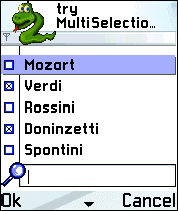
\includegraphics[width=\screenwidth]{checkbox-list}
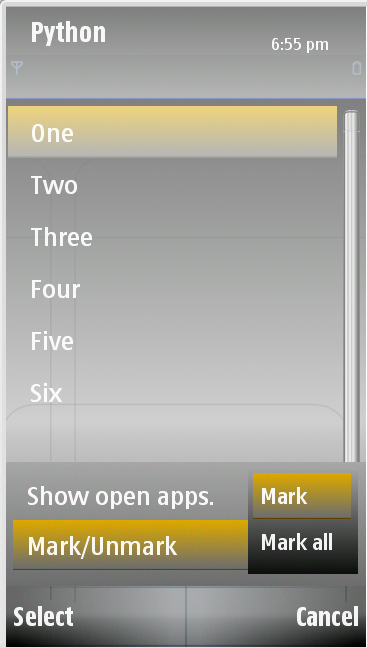
\includegraphics[width=\screenwidth]{markable-list}
\caption{Examples of a checkbox list (left) and a markable list (right)}
\label{fig:checkbox-and-markable-list}
\end{figure}

\subsection{Application Type}
\label{subsec:application}
A single implicit instance of this type always exists when \module{appuifw} 
module is present and can be referred to with the name \code{app}. New 
instances cannot be created by a Python program.

\begin{classdesc*}{Application}
Instances of \class{Application} type have the following attributes:

\begin{memberdesc}[Application]{body}
The UI control that is visible in the application's main window. Currently 
either \class{Text}, a \class{Listbox} object, \class{Canvas}, or 
\code{None}.
\end{memberdesc}

\begin{memberdesc}[Application]{directional_pad}
A boolean flag which controls the appearance of a virtual 4-way directional pad
that is displayed either at the bottom of the screen or on the right hand corner
depending on the orientation when using a Canvas. This is enabled by default on
devices that do not have a physical left and right soft key. This value is 
ignored on other devices, hence setting it to either True or False will have no effect.

Set it to \code{True} to enable 4-way directional pad and \code{False} to disable it.
\end{memberdesc}

\begin{memberdesc}[Application]{exit_key_handler}
A callable object that is called when the user presses the Exit softkey. 
Setting \member{exit_key_handler} to \code{None} sets it back to the 
default value.
\end{memberdesc}

\begin{memberdesc}[Application]{focus}
A callable object that is called with integer as parameter (0 = focus lost, 
1 = focus regained) when the application receives focus or it is switched to 
background. Focus is received e.g. when the application is switched from 
background to foreground or when the focus is regained from screensaver. 
Similarly when the screensaver is displayed, focus is lost.

Examples:
\begin{verbatim}
>>> import appuifw
>>> def cb(fg):
...   if(fg):
...     print "foreground"
...   else:
...     print "background"
...
>>> appuifw.app.focus=cb
>>> # switch to background, following text is printed from callback:
>>> background
>>> # switch to foreground, following text is printed from callback:
>>> foreground
\end{verbatim}

\begin{notice}
An improper callback can cause adverse effects. If you, for example,
define a callback which takes no parameters you will receive
never-ending \exception{TypeError} exceptions on the Nokia 6600.
\end{notice}

\end{memberdesc}

\begin{memberdesc}[Application]{menu}
This is a list of the following kinds of items:
\begin{itemize}
\item \code{(title, callback)} which creates a regular menu item
\item \code{(title, ((title, callback)\optional{...}))} which creates a submenu
\end{itemize}

\var{title} (Unicode) is the name of the item and \var{callback} the associated callable object. 
The maximum allowed number of items in a menu, or items in a submenu,
or submenus in a menu is 30.

Example:
\begin{verbatim}
appuifw.app.menu = [(u"Item 1", item1),
                    (u"Submenu 1", 
                        ((u"Subitem 1", subitem1),
                         (u"Subitem 2", subitem2)))]
\end{verbatim}
\end{memberdesc}

\begin{memberdesc}[Application]{orientation}
The orientation of the application. The orientation of the application can be 
one of the following values: \code{'automatic'} (this is the default value), 
\code{'portrait'} or \code{'landscape'}.
\end{memberdesc}

\begin{memberdesc}[Application]{screen}
The screen area used by an application. See \figurename~\ref{fig:alternate-uilayouts} for
example screens. The appearance of the application on the screen can
be affected by setting one of the following values: \code{'normal'},
\code{'large'} and \code{'full'}.

Examples:
\begin{verbatim}
appuifw.app.screen='normal'    # normal screen with title pane and softkey labels
appuifw.app.screen='large'     # only softkey labels visible
appuifw.app.screen='full'      # full screen mode on all devices
\end{verbatim}
\end{memberdesc}

\begin{memberdesc}[Application]{title}
The title of the application that is visible in the application's title
pane. Must be Unicode.
\end{memberdesc}

\begin{memberdesc}[Application]{track_allocations}
Set this to true if the interpreter should track all memory allocations and then
free the memory which was not explicitly released before application exit. The default
value of this attribute is true. As a consequence if there are any memory leaks in the
3rd party extension modules they will be released at the end. To check if there are
memory leaks(for debugging purposes) the following approach can be used :
\begin{verbatim}

appuifw.app.track_allocations = false

import my_extension
my_extension.do_something()

appuifw.app.track_allocations = true

\end{verbatim}
If the extension leaks memory then it will be reported at application exit.

\end{memberdesc}


Instances of \class{Application} type have the following methods:

\begin{methoddesc}[Application]{activate_tab}{index}
Activates the tab \var{index} counting from zero.
\end{methoddesc}

\begin{methoddesc}[Application]{full_name}{}
Returns the full name, in Unicode, of the native application in whose 
context the current Python interpreter session runs.
\end{methoddesc}

\begin{methoddesc}[Application]{layout}{layout_id}

Returns as a tuple the size and the position of the requested \code{layout_id}. 
The logical layouts are outlined partly in Figure \ref{fig:normal-uilayout}. The 
position is given from the top left corner. The \code{layout_id} can be one of 
the constants defined in module \module{appuifw}\footnote{Descriptions of the 
values are from the S60 SDK documentation \cite{S60Doc}.}:

\begin{datadesc}{EScreen} 
Screen.  
\end{datadesc}

\begin{datadesc}{EApplicationWindow} 
 Window that fills the entire screen.
\end{datadesc}

\begin{datadesc}{EStatusPane} 
Indicates common components for most of the applications.  
\end{datadesc}

\begin{datadesc}{EMainPane} 
The application main pane is used in all the applications.  
\end{datadesc}

\begin{datadesc}{EControlPane} 
Control pane.
\end{datadesc}

\begin{datadesc}{ESignalPane} 
The signal pane is used to indicate signal strength.  
\end{datadesc}

\begin{datadesc}{EContextPane} 
The context pane is used to indicate an active application.
\end{datadesc}

\begin{datadesc}{ETitlePane} 
Used to indicate the subject or the name of the main pane content. 
\end{datadesc}

\begin{datadesc}{EBatteryPane} 
The battery pane is used to indicate battery strength.  
\end{datadesc}

\begin{datadesc}{EUniversalIndicatorPane} 
The universal indicator pane is used to indicate items that require the user's 
attention while browsing applications. 
\end{datadesc}

\begin{datadesc}{ENaviPane} 
The navi pane is used to indicate navigation within an application, to provide 
context sensitive information to the user while entering or editing data, or to 
show additional information.  
\end{datadesc}

\begin{datadesc}{EFindPane} 
A fixed find pane is used with lists instead of the find pop-up window.  
\end{datadesc}

\begin{datadesc}{EWallpaperPane} 
Wallpaper pane.  
\end{datadesc}

\begin{datadesc}{EIndicatorPane} 
The universal indicator pane is used to indicate items that require the user's 
attention while browsing applications.  
\end{datadesc}

\begin{datadesc}{EAColumn} 
Used generally to display small sized graphics or heading texts.  
\end{datadesc}

\begin{datadesc}{EBColumn} 
Used generally to display large sized icons or heading texts.  
\end{datadesc}

\begin{datadesc}{ECColumn} 
Used generally to display data entered by the user. Overlaps with the D column. 
\end{datadesc}

\begin{datadesc}{EDColumn} 
Used generally to display additional icons. Overlaps with the C column. 
\end{datadesc}

\begin{datadesc}{EStaconTop} 
Top part of status and control panes in landscape layout.  
\end{datadesc}

\begin{datadesc}{EStaconBottom} 
Bottom part of status and control panes in landscape layout.  
\end{datadesc}

\begin{datadesc}{EStatusPaneBottom} 
Bottom part of status pane in landscape layout.  
\end{datadesc}

\begin{datadesc}{EControlPaneBottom} 
Bottom part of control pane in landscape layout.  
\end{datadesc}

\begin{datadesc}{EControlPaneTop} 
Top part of control pane in landscape layout.  
\end{datadesc}

\begin{datadesc}{EStatusPaneTop} 
Top part of status pane in landscape layout.
\end{datadesc}

Example:
\begin{verbatim}
>>> import appuifw
>>> appuifw.app.layout(appuifw.EMainPane)
((176, 144), (0, 44))
>>> # size and position (x, y) of the main pane in Nokia N70
\end{verbatim}

\end{methoddesc}

\begin{methoddesc}[Application]{set_exit}{}
Requests a graceful exit from the application as soon as the current script 
execution returns.
\end{methoddesc}

\begin{methoddesc}[Application]{set_tabs}{tab_texts\optional{,callback=None}}
Sets tabs with given names on them in the navigation bar; 
\var{tab_texts} is a list of Unicode strings. When the users 
navigate between tabs, \var{callback} gets called with the index 
of the active tab as an argument. Tabs can be disabled by giving an empty or 
one-item \var{tab_texts} list.
\end{methoddesc}

\begin{methoddesc}[Application]{uid}{}
Returns the UID, in Unicode, of the native application in whose 
context the current Python interpreter session runs.
\end{methoddesc}

\end{classdesc*}

\subsection{Form Type}
\label{subsec:form}
\class{Form} implements a dynamically configurable, editable multi-field 
dialog. \class{Form} caters for advanced dialog use cases with requirements 
such as free selectability of the combination of fields, possibility of 
validating the user input, and automatically producing the contents of some 
dialog fields before allowing the closing of the dialog. 

\begin{classdesc}{Form}{fields\optional{, flags=0}}
Creates a \class{Form} instance.
\var{fields} is a list of \emph{field descriptors}: \code{(label, type\optional{, value})} where

\var{label} is a Unicode string

\var{type} is one of the following strings: 
\code{'text'}, \code{'number'}, \code{'date'}, \code{'time'}, \code{'combo'}
or \code{'float'}

\var{value}, depending on \var{type}: Unicode string, numeric, float (seconds 
since Unix epoch rounded down to the nearest local midnight), float (seconds 
since local midnight), \code{([choice_label ...], index)} of float. For 
\code{'float'} \var{type} the initial value setting might not be shown in the 
UI.
\end{classdesc}

\class{Form} can also be configured and populated after construction. The 
configuration flags are visible as an attribute. \class{Form} implements 
the list protocol that can be used for setting the form fields, as well as 
obtaining their values after the dialog has been executed.

Instances of \class{Form} type have the following attributes:

\begin{memberdesc}[Form]{flags}
This attribute holds the values of the various configuration flags. 
Currently supported flags are:

\begin{datadesc}{FFormEditModeOnly}
When this flag is set, the form remains in edit mode while \method{execute} 
runs.
\end{datadesc}

\begin{datadesc}{FFormViewModeOnly}
When this flag is set, the form cannot be edited at all.
\end{datadesc}

\begin{datadesc}{FFormAutoLabelEdit}
This flag enables support for allowing the end-users to edit the labels of 
the form fields.
\end{datadesc}

\begin{datadesc}{FFormAutoFormEdit}
This flag enables automatic support for allowing the end-users to add and 
delete the form fields. Note that this is an experimental feature and is not 
guaranteed to work with all SDK versions.
\end{datadesc}

\begin{datadesc}{FFormDoubleSpaced}
When this flag is set, double-spaced layout is applied when the form is 
executed: one field takes two lines, as the label and the value field are on 
different lines.
\end{datadesc}
\end{memberdesc}

\begin{memberdesc}[Form]{menu}
A list of \code{(title, callback)} pairs, where 
each pair describes an item in the form's menu bar that is active while the 
dialog is being executed. \var{title} (Unicode) is the name of 
the item and \var{callback} the associated callable object.
\end{memberdesc}

\begin{memberdesc}[Form]{save_hook}
This attribute can be set to a callable object that receives one argument 
and returns a Boolean value. It gets called every time the users want to 
save the contents of an executing \class{Form} dialog. A candidate list for 
new form content - a list representing the currently visible state of the 
UI - is given as an argument. The list can be modified by 
\member{save_hook}. If \member{save_hook} returns \code{True}, the 
candidate list is set as the new contents of the form. Otherwise, the form 
UI is reset to reflect the field list contained in \class{Form} object.
\end{memberdesc}

Instances of \class{Form} type have the following methods:

\begin{methoddesc}[Form]{execute}{}
Executes the dialog by making it visible on the UI.
\end{methoddesc}

\begin{methoddesc}[Form]{insert}{index, field_descriptor}
Inserts the field descriptor into the \class{Form} before the given \var{index}.
\end{methoddesc}

\begin{methoddesc}[Form]{pop}{}
Removes the last field descriptor from the \class{Form} and returns it.
\end{methoddesc}

\begin{methoddesc}[Form]{length}{}the number of field descriptors in the form.
\end{methoddesc}

The subscript notation \code{f[i]} can be used to access or modify the
i-th element of the form \code{f}. Same limitations as discussed above
in the context of the flag \constant{FFormAutoFormEdit} apply to
modifying a form while it is executing. The ability to change the
schema of a form while it is executing is an experimental feature.

\subsection{Text Type}
\label{subsec:mylabel5}
\class{Text} is a text editor UI control. For examples on the options 
available with \class{Text}, see Figure \ref{fig:text-styles}.

\begin{figure}[htbp]
\centering
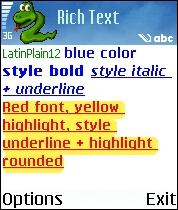
\includegraphics[width=\screenwidth]{text-styles-1}
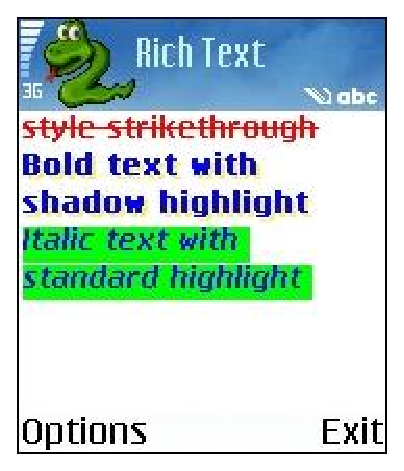
\includegraphics[width=\screenwidth]{text-styles-2}
\caption{Examples of the options available for Text type}
\label{fig:text-styles}
\end{figure}

Instances of \class{Text} type have the following attributes:

\begin{memberdesc}[Text]{color}
The color of the text. \code{color} supports the same color representation 
models as the \module{graphics} module. For the supported color 
representation models, see Section \ref{sec:graphics}.
\end{memberdesc}

\begin{memberdesc}[Text]{focus}
A Boolean attribute that indicates the focus state of the control. Editor 
control also takes the ownership of the navigation bar, and this feature is 
needed to enable the usage of this control in applications that use the 
navigation bar - for example, navigation tabs.
\end{memberdesc}

\begin{memberdesc}[Text]{font} 
The font of the text. There are two possible ways to set this attribute:

\begin{itemize}

\item Using a supported Unicode font, for example \code{u"Latin12"}. Trying to set a font which is not supported by the device has no effect. A list of supported fonts can be retrieved by using \function{appuifw.available_fonts}.

Example, setting font:
\begin{verbatim}
t = appuifw.Text()
t.font = u"albi17b" # sets font to Albi 17 bold
t.font = u"LatinPlain12" # sets font to Latin Plain 12
\end{verbatim}
\item Using one of the default device fonts that are associated with the following labels (plain strings):
\code{'annotation', 'title', 'legend', 'symbol', 'dense', 'normal'.}

Example, setting font: 
\begin{verbatim}
t.font = "title" # sets font to the one used in titles
\end{verbatim}

Example, checking the currently set font: 
\begin{verbatim}
unicodeFont = t.font
\end{verbatim}
\end{itemize}

The attribute value retrieved is always a Unicode string. If the font has 
been set with a label, for example, \code{'title'}, the attribute will 
retrieve the font associated with that label. 
\end{memberdesc}

\begin{memberdesc}[Text]{highlight_color}
The highlight color of the text. \code{highlight_color} supports the 
same color representation models as the \module{graphics} module. For the 
supported color representation models, see Section \ref{sec:graphics}.
\end{memberdesc}

\begin{memberdesc}[Text]{style}
The style of the text. The flags for this attribute are defined in the 
\module{appuifw} module. These flags can be combined by using the binary 
operator \code{|}. The flags can be divided into two types: text style 
and text highlight. Text style flags can be freely combined with each other. 
However, one or more text style flags can be combined with only one text 
highlight flag. The flags are:

Text style:

\begin{datadesc}{STYLE_BOLD} 
Enables bold text.
\end{datadesc}

\begin{datadesc}{STYLE_UNDERLINE}
Enables underlined text.
\end{datadesc}

\begin{datadesc}{STYLE_ITALIC} 
Enables italic text.
\end{datadesc}

\begin{datadesc}{STYLE_STRIKETHROUGH } 
Enables strikethrough.
\end{datadesc}

Text highlight:

\begin{datadesc}{HIGHLIGHT_STANDARD}
Enables standard highlight.
\end{datadesc}

\begin{datadesc}{HIGHLIGHT_ROUNDED}
Enables rounded highlight.
\end{datadesc}

\begin{datadesc}{HIGHLIGHT_SHADOW}
Enables shadow highlight.
\end{datadesc}

Only one highlight is allowed to be used at once. Therefore, it is possible 
to combine only one highlight with one or more text styles.

Examples:
\begin{verbatim}
t = appuifw.Text()

# These and other similar values and combinations are valid:
t.style = appuifw.STYLE_BOLD
t.style = appuifw.STYLE_UNDERLINE
t.style = appuifw.STYLE_ITALIC
t.style = appuifw.STYLE_STRIKETHROUGH
t.style = (appuifw.STYLE_BOLD|
	   appuifw.STYLE_ITALIC|
	   appuifw.STYLE_UNDERLINE)

# These values are valid:
t.style = appuifw.HIGHLIGHT_STANDARD
t.style = appuifw.HIGHLIGHT_ROUNDED
t.style = appuifw.HIGHLIGHT_SHADOW

# This combination is NOT valid:
# Invalid code, do not try!
t.style = (appuifw.HIGHLIGHT_SHADOW|appuifw.HIGHLIGHT_ROUNDED)
\end{verbatim}
\end{memberdesc}

Instances of \class{Text} type have the following methods:

\begin{methoddesc}[Text]{add}{text}
Inserts the Unicode string \var{text} to the current cursor position.
\end{methoddesc}

\begin{methoddesc}[Text]{bind}{event_code, callback}
Binds the callable Python object \var{callback} to event
\var{event_code}. The key codes are defined in 
the \module{key_codes} library module. The call 
\code{bind(event_code, None)} clears an 
existing binding. In the current implementation the event is always
passed also to the underlying native UI control.
\end{methoddesc}

\begin{methoddesc}[Text]{clear}{}
Clears the editor.
\end{methoddesc}

\begin{methoddesc}[Text]{delete}{\optional{pos=0, length=len()}}
Deletes \var{length} characters of the text held by the editor control, 
starting from the position \var{pos}.
\end{methoddesc}

\begin{methoddesc}[Text]{get_pos}{}
Returns the current cursor position.
\end{methoddesc}

\begin{methoddesc}[Text]{len}{}
Returns the length of the text string held by the editor control.
\end{methoddesc}

\begin{methoddesc}[Text]{get}{\optional{pos=0, length=len()}}
Retrieves \code{length} characters of the text held by the editor control, 
starting from the position \var{pos}.
\end{methoddesc}

\begin{methoddesc}[Text]{set}{text}
Sets the text content of the editor control to Unicode string 
\var{text}.
\end{methoddesc}

\begin{methoddesc}[Text]{set_pos}{cursor_pos}
Sets the cursor to \var{cursor_pos}.
\end{methoddesc}

\subsection{Listbox Type}
\label{subsec:listbox}

\begin{figure}[htbp]
\centering
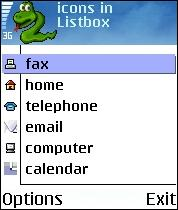
\includegraphics[width=\screenwidth]{listbox-with-icons}
\caption{Listbox with icons}
\label{fig:listbox-with-icons}
\end{figure}

An instance of this UI control type is visible as a listbox, also known as a 
list in Symbian, that can be configured to be a single-line item or a 
double-item listbox. Figure \ref{fig:listbox-with-icons} shows a single-line 
item Listbox with icons. For more information on the MBM and MIF formats, 
see Section \ref{subsec:icon}.

\begin{classdesc}{Listbox}{list, callback}
Creates a \class{Listbox} instance. A callable object 
\var{callback} gets called when a listbox selection has been 
made. \code{list} defines the content of the listbox and can be one of the 
following:

\begin{itemize}
\item A normal (single-line item) listbox: a list of Unicode strings, for example \code{[unicode_string item1, unicode_string item2]}
\item A double-item listbox: a two-element tuple of Unicode strings , for example \code{[(unicode_string item1, unicode_string item1description), (unicode_string item2, unicode_string item2description)]}
\item A normal (single-line item) listbox with graphics: a two-element tuple consisting of a Unicode string and an \class{Icon} object, for example \code{[(unicode_string item1, icon1), (unicode_string item2, icon2)]}.
\item A double-item listbox with graphics: a three-element tuple consisting of two Unicode strings and one \class{Icon} object, for example \code{[(unicode_string item1, unicode_string item1description, icon1), (unicode_string item2, unicode_string item2description, icon2)]}
\end{itemize}

Example: To produce a normal (single-line item) listbox with graphics:
\begin{verbatim}
icon1 = appuifw.Icon(u"z:\\resource\\apps\\avkon2.mbm", 28, 29)
icon2 = appuifw.Icon(u"z:\\resource\\apps\\avkon2.mbm", 40, 41)
entries = [(u"Signal", icon1),
           (u"Battery", icon2)]
lb = appuifw.Listbox(entries, lbox_observe)
\end{verbatim}
\end{classdesc}

\begin{notice}[note]
Known issue: Using this widget in large/full screen mode results in an unrefreshed area at the bottom of the screen.
\end{notice}

Instances of \class{Listbox} type have the following methods and properties:

\begin{methoddesc}[Listbox]{bind}{event_code, callback}
Binds the callable Python object \var{callback} to event 
\var{event_code}. The key codes are defined in 
the \module{key_codes} library module. The call
\code{bind(event_code, None)} clears an 
existing binding. In the current implementation the event is always passed 
also to the underlying native UI control.
\end{methoddesc}

\begin{methoddesc}[Listbox]{current}{}
Returns the currently selected item's index in the \class{Listbox}.
\end{methoddesc}

\begin{methoddesc}[Listbox]{set_list}{list\optional{, current}}
Sets the \class{Listbox} content to a list of Unicode strings or a
list of tuples of Unicode strings. The accepted structures of \var{list} are the
same as in the \class{Listbox} constructor. The optional argument \var{current} is the index of the focused list item.
\end{methoddesc}

\begin{memberdesc}[Listbox]{size}
The size of the \class{Listbox} as a tuple (width, height) - Read only.
\end{memberdesc}

\begin{memberdesc}[Listbox]{position}
The coordinates (as a tuple) of the top left corner of the \class{Listbox} -
Read only.
\end{memberdesc}

\subsection{Icon Type}
\label{subsec:icon}
An instance of \class{Icon} type encapsulates an icon to be used together 
with a \class{Listbox} instance. Note that currently \class{Icon} can only 
be used with \class{Listbox} (see Section \ref{subsec:listbox}).

MBM is the native Symbian OS format used for pictures. It is a
compressed file format where the files can contain several bitmaps and
can be referred to by a number. An \code{.mbg} file is the header file
usually associated with an \code{.mbm} file, which includes symbolic
definitions for each bitmap in the file. For example, an
\file{avkon.mbm} file has an associated index file called
\file{avkon.mbg}, which is included in S60 SDKs. For more information
on the MBM format and the bitmap converter tool, see \cite{S60Doc} and
search the topics with the key term "How to provide Icons"; this topic
also points you to the Bitmap Converter tool that can be used for
converting bitmaps into the MBM format.

\begin{classdesc}{Icon}{filename, bitmap, bitmapMask}
Creates an icon. \var{filename} is a Unicode file name and must 
include the whole path. Note that MBM is the only file formats supported.
\var{bitmap} and \var{bitmapMask} are integers that represent the index of 
the icon and icon mask inside that file respectively.
\end{classdesc}

Example: The following builds an icon with the standard signal symbol:
\begin{verbatim}
icon = appuifw.Icon(u"z:\\resource\\apps\\avkon2.mbm", 28, 29)
\end{verbatim}

\subsection{Content_handler Type}
\label{subsec:content}

An instance of \class{Content_handler} handles data content by its MIME 
type.

\begin{classdesc}{Content_handler}{\optional{callback}}
Creates a \class{Content_handler} instance. A Content_handler handles
data content by its MIME type. The optional
\var{callback} is called when the embedded handler application 
started with the \method{open} method finishes. 
\end{classdesc}

Instances of \class{Content_handler} type have the following methods:

\begin{methoddesc}[Content_handler]{open}{filename}
Opens the file \var{filename} (Unicode) in its handler 
application if one has been registered for the particular MIME type. The 
handler application is embedded in the caller's thread. The call to this 
function returns immediately. When the handler application finishes, the 
\var{callback} that was given to the \class{Content_handler} 
constructor is called.
\end{methoddesc}

\begin{methoddesc}[Content_handler]{open_standalone}{filename}
Opens the file \var{filename} (Unicode) in its handler 
application if one has been registered for the particular MIME type. The 
handler application is started in its own process. The call to this function 
returns immediately. Note that \var{callback} is not called for 
applications started with this method.
\end{methoddesc}

\subsection{Canvas Type}
\label{subsec:canvas}
\class{Canvas} is a UI control that provides a drawable area on the screen 
and support for handling raw key events. \class{Canvas} supports the 
standard drawing methods that are documented in Section \ref{sec:graphics}.

\begin{classdesc}{Canvas}{\optional{redraw_callback=None, event_callback=None,
                                  resize_callback=None}}
Constructs a \class{Canvas}. The optional parameters are callbacks
that are called when specific events occur. 

\note{Watch out for cyclic
references here. For example, if the callbacks are methods of an
object that holds a reference to the \class{Canvas}, a reference cycle
is formed that must be broken at cleanup time or the
\class{Canvas} will not be freed.}

\var{redraw_callback} is called whenever a part of the \class{Canvas} 
has been obscured by something, is then revealed, and needs to be
redrawn. This can typically happen, for example, when the user
switches away from the Python application and back again, or after
displaying a pop-up menu. The callback takes as its argument a
four-element tuple that contains the top-left and the bottom-right
corner of the area that needs to be redrawn. In many cases redrawing
the whole
\class{Canvas} is a reasonable option. 

\var{event_callback} is called whenever a raw key event is received or when a 
pointer event occurs(only on touch input supported devices).
There are three kinds of key events: \code{EEventKeyDown},
\code{EEventKey}, and \code{EEventKeyUp}. When a user presses a key 
down, events \code{EEventKeyDown} and \code{EEventKey} are generated. 
When the key is released, an \code{EEventKeyUp} event is generated.

Pointer events are generated by touch input supported devices. When the screen
is touched the \code{EButton1Down} event is generated, \code{EDrag} while the
finger/stylus is dragged across the screen and then \code{EButton1Up} when the
finger/stylus is lifted.

The argument to the \var{event_callback} is a dictionary that contains 
the following data:

For key events:
\begin{itemize}
\item \code{'type'}: one of \code{EEventKeyDown}, \code{EEventKey}, or 
\code{EEventKeyUp}
\item \code{'keycode'}: the keycode of the key
\item \code{'scancode'}: the scancode of the key
\item \code{'modifiers'}: the modifiers that apply to this key event
\end{itemize}

For pointer events:
\begin{itemize}
\item \code{'type'}: one of the several pointer events - \code{EButton1Up}, 
\code{EButton1Down}, \code{EDrag} etc..
\item \code{'modifiers'}: the modifiers that apply to this pointer event
\item \code{'pos'}: A tuple containing the x-y pointer co-ordinates
\end{itemize}

Each key on the keyboard has one or more scancodes and zero or more keycodes 
associated with it. A scancode represents the physical key itself and a 
keycode is the result of state-related operating system defined processing 
done on the key. For keys that correspond to a symbol in the current 
character set of the phone, the keycode is equal to the code of the 
corresponding symbol in that character set. For example, if you are using 
the Nokia Wireless Keyboard (SU-8W), pressing the key A will always produce 
the scancode 65 (ASCII code for an upper case A), but the keycode 
could be either 65 or 91 (ASCII code for a lower case A) depending on 
whether or not the Shift key is pressed or Caps Lock is active. 

The \module{key_codes} module contains definitions for the keycodes and 
scancodes. See \figurename~\ref{fig:keyboard} for the codes of the most 
common keys on the phone keypad. 

Some keys are handled in a special way:

\begin{itemize}
\item A short press of the Edit key causes it to stay down, meaning that no \code{EEventKeyUp} event is sent. The event is only sent after a long press.
\item Detecting presses of the Voice tags key or the Power key is not supported.
\item If the right softkey is pressed, the \code{appuifw.app.exit_key_handler} callback is always executed.
\end{itemize}

There is no way to prevent the standard action of the Hang-up key, the Menu 
key, the Power key or the Voice tags key from taking place.

\begin{figure}
\centering
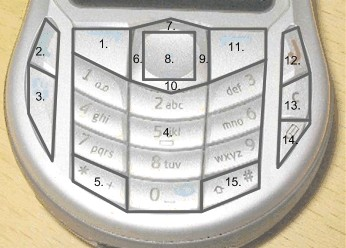
\includegraphics[width=5in]{6630keyboard}
%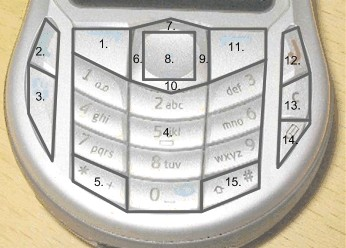
\includegraphics[width=3.60in,height=2.58in]{6630keyboard}
%\centerline{\includegraphics[width=3.60in,height=2.58in]{API_Reference_for_Python11.eps}} \par & 
\begin{tableiii}{lll}{textrm}{Key}{Keycode}{Scancode}
\lineiii{1.}{EKeyLeftSoftkey}{EScancodeLeftSoftkey}
\lineiii{2.}{EKeyYes}{EScancodeYes}
\lineiii{3.}{EKeyMenu}{EScancodeMenu}
\lineiii{4.}{EKey0...9}{EScancode0...9}
\lineiii{5.}{EKeyStar}{EScancodeStar}
\lineiii{6.}{EKeyLeftArrow}{EScancodeLeftArrow}
\lineiii{7.}{EKeyUpArrow}{EScancodeUpArrow}
\lineiii{8.}{EKeySelect}{EScancodeSelect}
\lineiii{9.}{EKeyRightArrow}{EScancodeRightArrow}
\lineiii{10.}{EKeyDownArrow}{EScancodeDownArrow}
\lineiii{11.}{EKeyRightSoftkey}{EScancodeRightSoftkey}
\lineiii{12.}{EKeyNo}{EScancodeNo}
\lineiii{13.}{EKeyBackspace}{EScancodeBackspace}
\lineiii{14.}{EKeyEdit}{EScancodeEdit}
\lineiii{15.}{EKeyHash}{EScancodeHash}
\end{tableiii}
\caption{Keycodes and scancodes for phone keys usable from Python applications}
\label{fig:keyboard}
\end{figure}

\var{resize_callback} is called when screen size is changed when the 
\class{Canvas} rect size has been changed. The callback takes as its argument a
two-element tuple that contains the new clientRect width and height. 

\end{classdesc}

Instances of \class{Canvas} type have the following methods:

\begin{methoddesc}[Canvas]{bind}{pointer_event, callable\optional{, ((x1, y1), (x2, y2))}}
This method can be used to listen to specific pointer events. The
\var{pointer_event} argument can be any one of the pointer events listed in the
\module{key_codes} module.

The most common pointer events are:

\begin{itemize}
\item \code{EButton1Down} - Pen down event 
\item \code{EButton1Up}   - Pen up event
\item \code{EDrag}        - Drag event (This event is only received when button1 is down)
\item \code{ESwitchOn}    - Switch on event caused by a screen tap.
\end{itemize}

\var{callable} is called when the pointer_event and the co-ordinate 
(if specified) criterion matches.

\var{((x1, y1), (x2, y2))} is an optional argument that can be passed to
specify the screen area to monitor for any specific pointer event. The two
co-ordinate tuple corresponds to the top-left and bottom-right points. This
argument will be ignored if the event is not a pointer event.

There are several ways in which bind can be used:

\begin{itemize}
\item \code{my_canv.bind(EButton1Up, callback)} - The callback is called when
EButton1Up event is generated anywhere in the canvas.

\item \code{my_canv.bind(EButton1Up, green_callback, ((x1, y1), (x2, y2)))} - The 
callback is called when the EButton1Up pointer event occurs inside the screen
area specified.

\item \code{my_canv.bind(EButton1Up, yellow_callback, ((x3, y3), (x4, y4)))} - 
Registers another callback for a different region but for the same pointer
event. When two screen areas overlap, the callback registered last will be
called when pointer events occur in the intersected region. 

\item \code{my_canv.bind(EButton1Up, callback3, ((x1, y1), (x2, y2)))} - If the
pointer event and the screen area to be monitored are the same, the callback
passed will replace the old callback already registered. 

\item \code{my_canv.bind(EButton1Up, None, ((x1, y1), (x2, y2)))} - If the pointer
event and the screen area to be monitored are the same, and the callback passed
is None, the callback registered previously is cleared.

\item \code{my_canv.bind(EButton1Up, None)} - All callbacks previously registered
for this pointer event are cleared, regardless of whether it was for a specific
screen area or for the entire canvas.
\end{itemize}

\begin{figure}
\centering
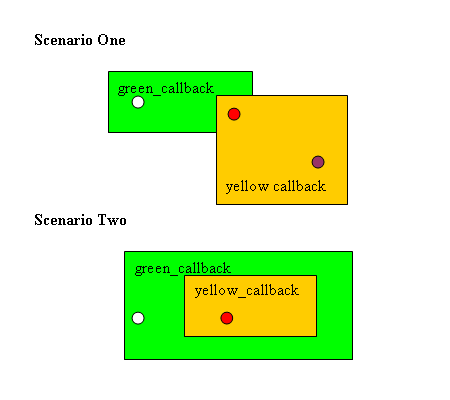
\includegraphics[width=5in]{bind-scenarios}
\caption{Canvas bind scenarios}
\label{fig:bind-scenarios}
\end{figure}

Clicking on the white spot should result in \code{green_callback} to be called. 
Clicking on the red spot should result in \code{yellow_callback} to be called in both
the scenarios shown above provided the \code{yellow_callback} was registered last. 
Clicking on the purple spot should result in \code{yellow_callback} to be called.

\end{methoddesc}

\begin{methoddesc}[Canvas]{begin_redraw}{\optional{((x1, y1), (x2, y2))}}
This is an explicit function that can be used to signal the window server that 
"I'm about to redraw this area". This method tells the window server that the 
window is about to respond to the last redraw event by redrawing the specified 
rectangle. This causes the window server to clear the rectangle, and remove it 
from the invalid region.
The optional co-ordinates x1, y1, x2, y2 should be the rectangle that has to be marked
for redrawing.

After the redraw is complete the application should call end_redraw().

\note{The begin_redraw and end_redraw methods should not be called inside the
redraw callback function.}

Couple of FAQs on redraw/non-redraw drawing:

Question: What is non-redraw drawing?
\begin{itemize}
\item "Non-redraw drawing" is any canvas/graphics drawing operation performed 
outside of begin_redraw()/end_redraw().
\end{itemize}

Question: What should applications do instead of non-redraw drawing?
\begin{itemize}
\item "Redraw drawing" is any drawing delimited by begin_redraw()/end_redraw().
\end{itemize}

Question: Why is non-redraw drawing bad for performance?
\begin{itemize}
\item The window server caches drawing operations in the redraw store.
Delimiting drawing with begin_redraw()/end_redraw() allows window server to 
efficiently manage drawing operations. 

If applications perform drawing operations outside begin_redraw/end_redraw,
window server cannot cull drawing operations from its cache of drawing 
operations, because it cannot know whether a set of drawing operations has 
been superceded by a new set.
In this scenario every frame of drawing that is done on a non-redraw drawing window 
will become slower and slower as it draws all the drawing operations for the 
entire history of the window (well actually up until the last begin_redraw/end_redraw 
for the whole window).

If an application performs begin_redraw/end_redraw, it tells the window server 
that it can throw away any old drawing operations it had for the area of the 
window specified in the redraw, thus allowing for more optimal management of 
drawing operations.
\end{itemize}

Question: What are the changes required for redraw drawing?
\begin{itemize}
\item Applications should delimit their drawing with begin_redraw()/end_redraw() 
- i.e. they should replace non-redraw drawing with redraw drawing. Sometimes, 
this is as straight forward as adding these calls to existing rendering code.
In other cases (where the application has been drawing using "incremental updates" 
to the window, the application drawing code would need to be reworked to perform a 
full refresh of the area redrawn for the rect provided in begin_redraw(rect).
\end{itemize}
\end{methoddesc}

\begin{methoddesc}[Canvas]{end_redraw}{}
Ends the current redraw. This function should be called when redrawing is complete.
\end{methoddesc}


Instances of \class{Canvas} type have the following attribute:

\begin{memberdesc}[Canvas]{size}
A two-element tuple that contains the current width and height of the 
\class{Canvas} as integers.
\end{memberdesc}

Instances of \class{Canvas} type have the same standard drawing methods 
that are documented in Section \ref{sec:graphics}.

\subsection{InfoPopup Type}
\label{subsec:infopopup}

An instance of \class{InfoPopup} type encapsulates an UI tip widget. This widget 
can be placed on top of other widgets to provide e.g. usage information to the 
user. The widget disappears as soon as the device's user presses any key or when 
the timer behind the \class{InfoPopup} is triggered.

\begin{classdesc}{InfoPopup}{}
Creates an \class{InfoPopup}.
\end{classdesc}

\begin{methoddesc}[InfoPopup]{show}{text, \optional{(x_coord, y_coord), 
time_shown, time_before, alignment}}
Show \var{text} (Unicode) in the \class{InfoPopup}. The optional parameters are 
the location (a tuple from the upper left corner), the time the popup is 
visible, \var{time_shown} (in milliseconds), the time before the popup, 
\var{time_before} (in milliseconds) and the alignment of the popup.

The default values are: the coordinates \code{(0, 0)}, \var{time_shown} 5 
seconds, \var{time_before} 0 seconds and for the alignment 
\code{appuifw.EHLeftVTop}.

The \var{alignment} can be one of the constants defined in module 
\code{appuifw}\footnote{Descriptions of the values are from the S60 SDK 
documentation \cite{S60Doc}.}:

\begin{datadesc}{EHLeftVTop} 
Object is left and top aligned. 
\end{datadesc}

\begin{datadesc}{EHLeftVCenter} 
Object is left aligned and centred vertically. 
\end{datadesc}

\begin{datadesc}{EHLeftVBottom} 
Object is left aligned and at the bottom. 
\end{datadesc}

\begin{datadesc}{EHCenterVTop} 
Object is centre aligned horizontally and at the top. 
\end{datadesc}

\begin{datadesc}{EHCenterVCenter} 
Object is centred horizontally and vertically. 
\end{datadesc}

\begin{datadesc}{EHCenterVBottom} 
Object is centred horizontally and at the bottom. 
\end{datadesc}

\begin{datadesc}{EHRightVTop} 
Object is right and top aligned. 
\end{datadesc}
 
\begin{datadesc}{EHRightVCenter} 
Object is right aligned and centred vertically. 
\end{datadesc}

\begin{datadesc}{EHRightVBottom} 
Object is right aligned and at the bottom. 
\end{datadesc}

\end{methoddesc}

\begin{methoddesc}[InfoPopup]{hide}{}
Hides the popup immediately.
\end{methoddesc}

Example:

\begin{verbatim}
>>> import appuifw
>>> i=appuifw.InfoPopup()
>>> i.show(u"Here is the tip.", (0, 0), 5000, 0, appuifw.EHRightVCenter)
>>>
\end{verbatim}
